% !TeX spellcheck = en_US 
\documentclass[11pt]{article}

\usepackage{amssymb} % see: http://milde.users.sourceforge.net/LUCR/Math/mathpackages/amssymb-symbols.pdf
\usepackage{mathtools} % for extended mathematical symbols and more

% Page properties :
% See : https://tex.stackexchange.com/questions/36085/latex-without-pages
\usepackage{geometry}
\geometry{margin=16mm}


% fix for underlined text not hyphenating :
%\usepackage{soul} % use this
% then replace '\underline{}' with '\ul{}'

% To color text :
% see : https://en.wikibooks.org/wiki/LaTeX/Colors
\usepackage[dvipsnames]{xcolor} % use this
% then use one of these syntaxes :
% >\textcolor{declared-color}{text}
% >{\color{declared-color} text}

% Input file encoding :
\usepackage[utf8]{inputenc}     % makes accents not shit

% To use images : 
\usepackage{graphicx} % use this
\graphicspath{ {./IMG/} } % path midifier for storing images
% to include a picture, type this ('name' is without path or extention) :
% \includegraphics[width=0.5\textwidth]{name}

% Box : % width should be manually set
% \fbox{ \parbox{0.8\textwidth}{ text } }

% Espacement :
% \hfill \vfill
% \vspace{length} \hspace{length} % if ignored, use starred version or { \vspace*{length} }
% \phantom{text} 
% Indentation explicite :
% \indent et \noindent
\usepackage{parskip}

% Fractions :
% \frac{num}{denum}  % small text num/denum
% \dfrac{num}{denum} % normal text num/denum

% Coloring text: % works on text and math modes
% \textcolor{declared-color}{text}
% {\color{declared-color}some text}

% How to use references :
\usepackage{hyperref} % use this
% use '\hypertarget{some_label}{}', then
% and reference it with '\hyperlink{some_label}{some text}'
\hypersetup{
	colorlinks=true,    
	urlcolor=blue,
}

% To write prooftrees :
% see : http://www.pirbot.com/mirrors/ctan/macros/latex/contrib/ebproof/ebproof.pdf
%\usepackage{ebproof} % use this


% Verbatim blocks :
\usepackage{verbatim} % normal verbatim
\usepackage{fancyvrb} % for fancy boxed varbatims
\usepackage{parskip}

% For code
\usepackage{listings}
%\begin{lstlisting}
%Put your code he<re.
%\end{lstlisting}


\usepackage{color}

\definecolor{mylightgray}{rgb}{0.95,0.95,0.95}

\usepackage[super]{nth}

% Regulates \tableofcontents max depth
\setcounter{tocdepth}{2}

\usepackage{array}
\newcolumntype{L}[1]{>{\raggedright\let\newline\\\arraybackslash\hspace{0pt}}m{#1}}
\newcolumntype{C}[1]{>{\centering\let\newline\\\arraybackslash\hspace{0pt}}m{#1}}
\newcolumntype{R}[1]{>{\raggedleft\let\newline\\\arraybackslash\hspace{0pt}}m{#1}}

\usepackage{xcolor,colortbl}
\newcolumntype{a}{>{\columncolor{mylightgray}}l}

\usepackage{array}
\setlength\extrarowheight{4pt} % or whatever amount is appropriate

\lstset{ 
	backgroundcolor=\color{mylightgray},   % choose the background color; you must add \usepackage{color} or \usepackage{xcolor}; should come as last argument
	basicstyle=\small,        % the size of the fonts that are used for the code
	breakatwhitespace=false,         % sets if automatic breaks should only happen at whitespace
	breaklines=true,                 % sets automatic line breaking
	captionpos=b,                    % sets the caption-position to bottom
	commentstyle=\color{mygreen},    % comment style
	deletekeywords={...},            % if you want to delete keywords from the given language
	escapeinside={\%*}{*)},          % if you want to add LaTeX within your code
	extendedchars=true,              % lets you use non-ASCII characters; for 8-bits encodings only, does not work with UTF-8
	firstnumber=1,                % start line enumeration with line 1000
	frame=single,	                   % adds a frame around the code
	keepspaces=true,                 % keeps spaces in text, useful for keeping indentation of code (possibly needs columns=flexible)
	keywordstyle=\color{blue},       % keyword style
	%language=Java,                 % the language of the code
	morekeywords={},            % if you want to add more keywords to the set
	numbers=none,                    % where to put the line-numbers; possible values are (none, left, right)
	numbersep=5pt,                   % how far the line-numbers are from the code
	numberstyle=\tiny\color{mygray}, % the style that is used for the line-numbers
	rulecolor=\color{black},         % if not set, the frame-color may be changed on line-breaks within not-black text (e.g. comments (green here))
	showspaces=false,                % show spaces everywhere adding particular underscores; it overrides 'showstringspaces'
	showstringspaces=false,          % underline spaces within strings only
	showtabs=false,                  % show tabs within strings adding particular underscores
	stepnumber=2,                    % the step between two line-numbers. If it's 1, each line will be numbered
	stringstyle=\color{mygreen},     % string literal style
	tabsize=2,	                   % sets default tabsize to 2 spaces
	title=\lstname                   % show the filename of files included with \lstinputlisting; also try caption instead of title
}
\usepackage[english]{babel}
\usepackage{lipsum}
\usepackage{multirow,booktabs} % https://jdhao.github.io/2019/08/27/latex_table_with_booktabs/

\newcounter{codeID}[section]
\newcommand{\nextcodeID}{\refstepcounter{codeID}\multirow{4}{*}{\thecodeID}}

\usepackage{longtable}

\newcommand{\degrees}[1]{#1$^{\circ}$}


%opening
\title{RPG Maker XP documentation}
\author{David Rodriguez Soares}


% first page
\begin{document}
\maketitle

\vspace{90mm}

\textbf{Privacy policy}

This is a confidential document and should not be distributed under any circumstance. \hyperref[sec:privacypolice]{Please click and read}.

\textbf{Abstract}

\lipsum[2-3]


\newpage

\begingroup
\hypersetup{linkcolor=black}
\tableofcontents
\endgroup

\newpage
\section{What this document is about}

This document holds information about how RPG Maker XP implements \textit{Events}, which is relevant in project PoGER's map/feature extraction effort.

Please read this document's \hyperref[sec:privacypolice]{Privacy Policy}.

As a result of the limited scope of PoGER and the limited time and information available to the author, the following documentation isn't complete and may not be accurate.

The information was obtained through the official RPG Maker XP built-in documentation, user content found on the internet (forum posts, videos) and the author's reverse-engineering work.

The following abbreviations may be present :
\begin{itemize}
	\item \textbf{RMXP} - RPG Maker XP
	\item \textbf{PE} - Pokemon Essentials
\end{itemize}



\section{Events}

An event, or more precisely a \textit{map event}, is a way to introduce elements with behavior, therefore bringing flexibility and dynamism into the game world.

Events have two aspects :
\begin{itemize}
	\item A GUI element
	\vspace{2mm}
	\begin{center}
		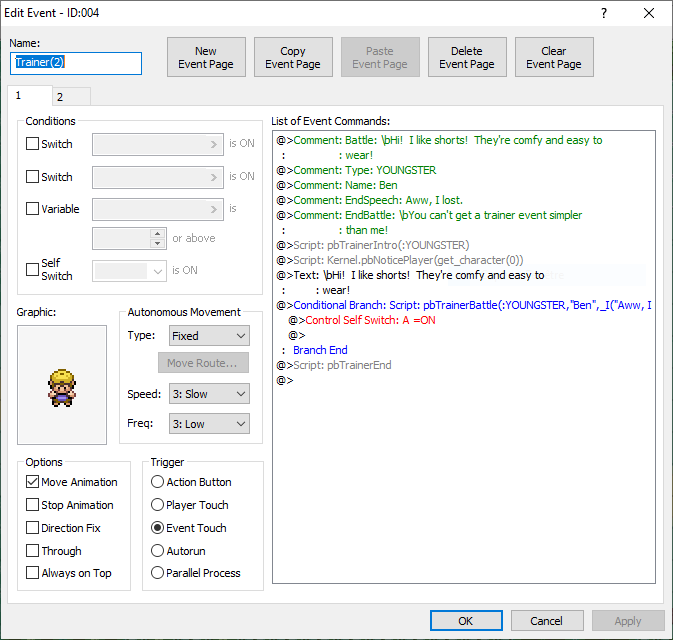
\includegraphics[width=0.75\textwidth]{Event} 
	\end{center}

	\item Its data class instance counterpart
	
	
\end{itemize}
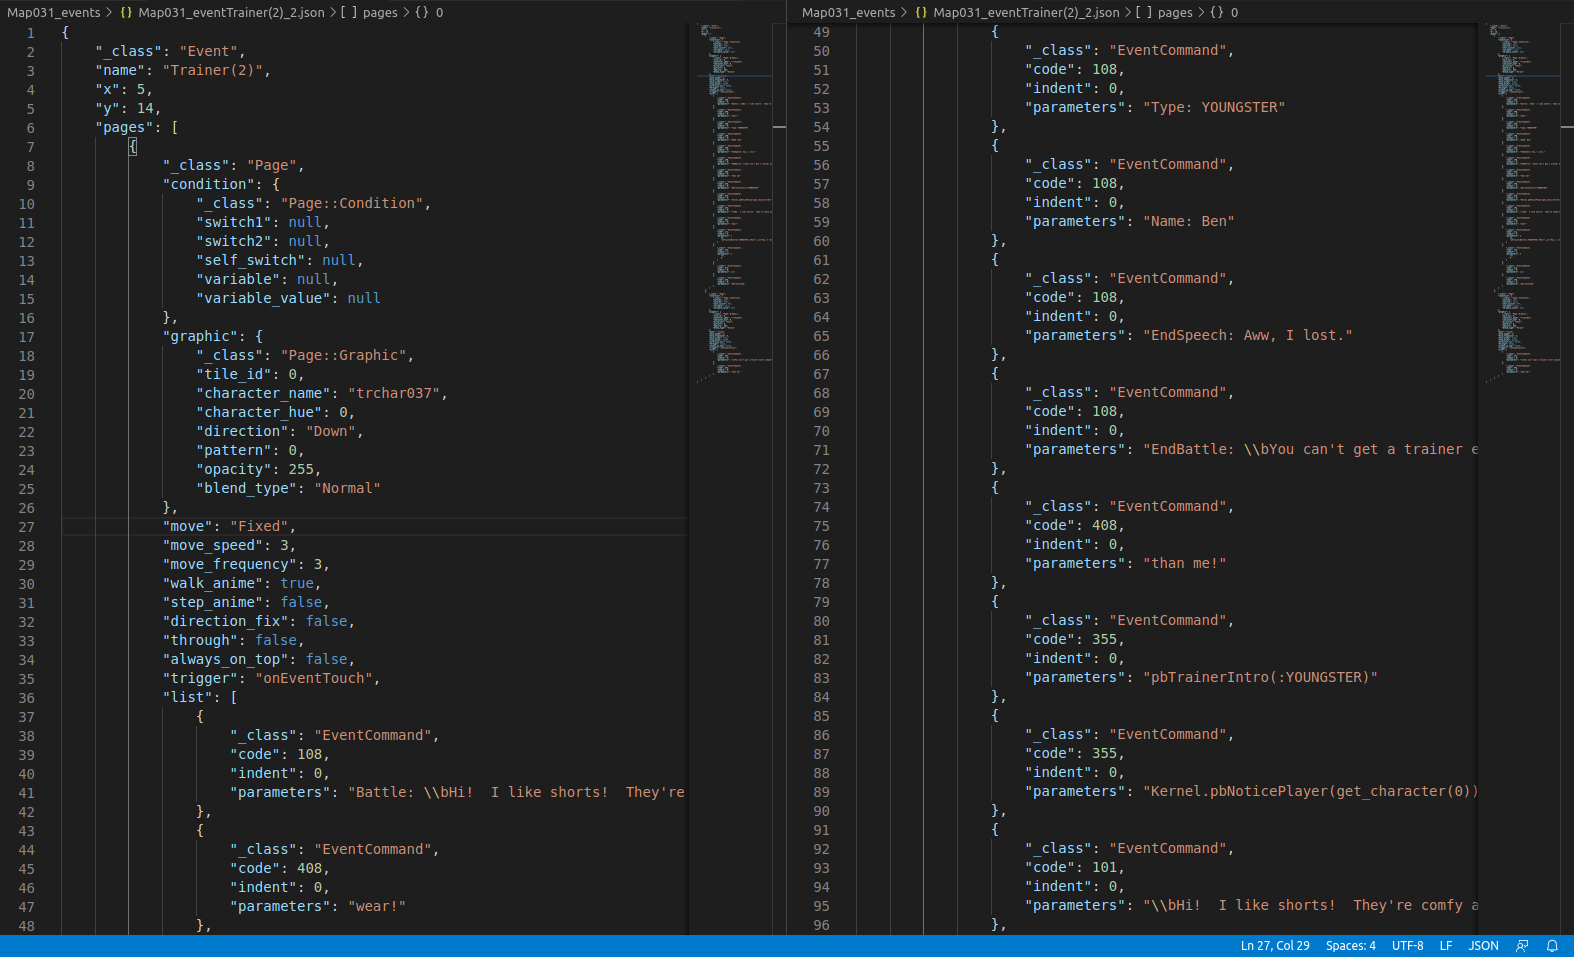
\includegraphics[width=\textwidth]{Event_json}


\subsection{Basic functionalities}

These are the easiest and most straightforward behavior to implement into an event :

\begin{itemize}
	\item Giving an element a \textit{sprite} (texture) : This is useful for objects capable of movement, NPCs, etc.
	
	\item \textit{Movement} : Select how the element moves with presets (speed, frequency, pattern, etc).
	
	\item \textit{Event commands} : Select the trigger for behavior and what the element does when triggered (movement, dialogue, etc) within the extensive command list.
\end{itemize}

\subsection{Advanced functionalities}

These require an understanding of conditional execution and scripting :

\begin{itemize}
	\item \textit{Conditional execution} : branching instructions based on the value of : global variables, global switches, self switches, script return, etc.
	
	\item \textit{Pages} : Allow to give an element different behavior depending on conditions.
	
	\item \textit{Move routes} : Define a sequence of movement commands to be executed.
	
	\item \textit{Script calls} : Call a script to be executed for more complex behavior, launching mini-games, retrieving data, etc.
\end{itemize}



\newpage
\section{Commands}

Although they are very similar in structure and use, a distinction is made between \verb|RPG::EventCommand| and \verb|RPG::MoveCommand|.

\textit{EventCommands} are the representation of elements present in the "List of Event Commands" in the GUI. They are the building block of event's behavior.

\textit{MoveCommands} are the representation of an individual movement the event is capable of, typically found in sequences \verb|RPG::MoveRoute| associated with a dedicated \textit{EventCommand}.

They both have, at least :
\begin{itemize}
	\item A \textit{code} : An integer that uniquely identifies the particular command.
	\item \textit{Parameters} : Depend on the particular command, can be empty, a variable, an object, or a list of objects.
\end{itemize}

Additionally, \textit{EventCommands} have an \textit{indent} integer value, tied to the layout visible in the "List of Event Commands" in the GUI.


\subsection{Methodology}

In order to successfully \textit{extract semantic from events}, it was decided that \textit{documenting} every command used in Pokemon Essentials and finding an appropriate (human-readable) \textit{representation} was the way forward.

% I tested a few table designs

%\begin{table}[h!]
%	\begin{center}
%		\caption{More columns.}
%		\label{tab:table1}
%		\begin{tabular}{l|c|r|l}
%			\textbf{Value 1} & \textbf{Value 2} & \textbf{Value 3} & \textbf{Value 4}\\ % <-- added & and content for each column
%			$\alpha$ & $\beta$ & $\gamma$ & $\delta$ \\ % <--
%			\hline
%			1 & 1110.1 & a & e\\ % <--
%			2 & 10.1 & b & f\\ % <--
%			3 & 23.113231 & c & g\\ % <--
%		\end{tabular}
%	\end{center}
%\end{table}

%\begin{tabular}{c l l}
%	\toprule
%	\multirow{3}{*}[-2mm]{1} & Description & \verb|RPG::MoveCommand| - "Move Down" \\
%	\cmidrule{2-3}
%	& Parameters & None \\
%	\cmidrule{2-3}
%	& Representation & "Move Down" \\ [1mm]
%	\toprule
%\end{tabular}

%\begin{tabular}{c a l}
%	\toprule
%	\multirow{3}{*}[-2mm]{1} & Description & \verb|RPG::MoveCommand| - "Move Down" \\
%	\cmidrule{2-3}
%	& Parameters & None \\
%	\cmidrule{2-3}
%	& Representation & "Move Down" \\ [1mm]
%	\toprule
%\end{tabular}

\subsection{Miscellaneous information}

Codes used in Pokemon Essentials 17.2 :
\begin{quote}
	0, 1, 2, 3, 4, 5, 6, 7, 8, 9, 10, 11, 12, 13, 14, 15, 16, 17, 18, 19, 20, 21, 22, 23, 24, 25, 26, 33, 34, 37, 38, 39, 40, 41, 42, 44, 101, 102, 104, 106, 108, 111, 112, 113, 115, 118, 119, 121, 122, 123, 125, 201, 202, 208, 209, 210, 221, 222, 223, 225, 231, 232, 235, 236, 241, 242, 247, 248, 249, 250, 314, 354, 355, 401, 402, 404, 408, 411, 412, 413, 655
\end{quote}

Implementation details :
\begin{itemize}
	\item \verb|RPG::MoveCommand| use range [1-45]
	
	\item \verb|RPG::EventCommand| use range [101-$x$], $x\geq 655$
	
	\item A "frame" is defined as $\dfrac{1}{20}$ second $\Rightarrow$ change into milliseconds $m=n*1000/20\equiv n*50$.
	
	\item Every event has an ID (integer $>0$). Actions that can affect other events can target the player using id \verb|-1| and the current event using id \verb|0|.
	
	\item Special variables : MapID, PartyMembers, \underline{Gold}, Steps, PlayTime, \textit{Timer}, SaveCount.
	
	They should all be read accessible. \underline{Underlined ones should also be write accessible}. \textit{Italic ones are probably not used}.
\end{itemize}

\vspace{4mm}
\subsection{List of commands}


\newpage
\setcounter{codeID}{-1}
{\small
\begin{tabular}{|c a l|}
	\hline
	\nextcodeID & Description & Nothing, empty command or end of the event command list \\
	& Parameters & None \\
	& Notes & Will not be represented \\
	& Representation & None \\
	\hline
	\nextcodeID & Description & \verb|RPG::MoveCommand| - Move to the South \\
	& Parameters & None \\
	& Notes & See footnote\footnotemark[1] \\
	& Representation & "Move, S" \\
	\hline
	\nextcodeID & Description & \verb|RPG::MoveCommand| - Move to the West \\
	& Parameters & None \\
	& Notes & See footnote\footnotemark[1] \\
	& Representation & "Move, W" \\
	\hline
	\nextcodeID & Description & \verb|RPG::MoveCommand| - Move to the East \\
	& Parameters & None \\
	& Notes & See footnote\footnotemark[1] \\
	& Representation & "Move, E" \\
	\hline
	\nextcodeID & Description & \verb|RPG::MoveCommand| - Move to the North \\
	& Parameters & None \\
	& Notes & See footnote\footnotemark[1] \\
	& Representation & "Move, N" \\
	\hline
	\nextcodeID & Description & \verb|RPG::MoveCommand| - Move to the SouthWest \\
	& Parameters & None \\
	& Notes & See footnote\footnotemark[1] \\
	& Representation & "Move, SW" \\
	\hline
	\nextcodeID & Description & \verb|RPG::MoveCommand| - Move to the SouthEast \\
	& Parameters & None \\
	& Notes & See footnote\footnotemark[1] \\
	& Representation & "Move, SE" \\
	\hline
	\nextcodeID & Description & \verb|RPG::MoveCommand| - Move to the NorthWest \\
	& Parameters & None \\
	& Notes & See footnote\footnotemark[1] \\
	& Representation & "Move, NW" \\
	\hline
	\nextcodeID & Description & \verb|RPG::MoveCommand| - Move to the NorthEast \\
	& Parameters & None \\
	& Notes & See footnote\footnotemark[1] \\
	& Representation & "Move, NE" \\
	\hline
	\nextcodeID & Description & \verb|RPG::MoveCommand| - Move at random (N,E,S,W) \\
	& Parameters & None \\
	& Notes & See footnote\footnotemark[1] \\
	& Representation & "Move, R" \\
	\hline
	\nextcodeID & Description & \verb|RPG::MoveCommand| - Move towards player \\
	& Parameters & None \\
	& Notes & See footnotes\footnotemark[1]\textsuperscript{,}\footnotemark[3] \\
	& Representation & "Move, TODO" \\
	\hline
\end{tabular}

\newpage
\begin{tabular}{|c a l|}
	\hline
	\nextcodeID & Description & \verb|RPG::MoveCommand| - Move away from player \\
	& Parameters & None \\
	& Notes & See footnotes\footnotemark[1]\textsuperscript{,}\footnotemark[3] \\
	& Representation & "Move, TODO" \\
	\hline
	\nextcodeID & Description & \verb|RPG::MoveCommand| - Take 1 step forward \\
	& Parameters & None \\
	& Notes & See footnote\footnotemark[1] \\
	& Representation & "Move, TODO" \\
	\hline
	\nextcodeID & Description & \verb|RPG::MoveCommand| - Take 1 step backward \\
	& Parameters & None \\
	& Notes & See footnote\footnotemark[1] \\
	& Representation & "Move, TODO" \\
	\hline
	\nextcodeID & Description & \verb|RPG::MoveCommand| - Jump to relative coordinates on the same map \\
	& Parameters & [2] - \textbf{0}:deltaX \verb|[signed integer]|, \ \textbf{1}:deltaY \verb|[signed integer]| \\
	& Notes &  \\
	& Representation & "Jump, TODO" \\
	\hline
	\nextcodeID & Description & \verb|RPG::MoveCommand| - Wait n seconds \\
	& Parameters & [1] - \textbf{0}:number of seconds to wait $n$ \verb|[integer|$\;\in \mathbb{N}^*$\verb|]| \\
	& Notes & Typically $n==2$, but values up to 15 were found in PE. \\
	& Representation & "Wait seconds, $n$" \\
	\hline
	\nextcodeID & Description & \verb|RPG::MoveCommand| - Turn towards South \\
	& Parameters & None \\
	& Notes & See footnote\footnotemark[2] \\
	& Representation & "Turn, S" \\
	\hline
	\nextcodeID & Description & \verb|RPG::MoveCommand| - Turn towards West \\
	& Parameters & None \\
	& Notes & See footnote\footnotemark[2] \\
	& Representation & "Turn, W" \\
	\hline
	\nextcodeID & Description & \verb|RPG::MoveCommand| - Turn towards East \\
	& Parameters & None \\
	& Notes & See footnote\footnotemark[2] \\
	& Representation & "Turn, E" \\
	\hline
	\nextcodeID & Description & \verb|RPG::MoveCommand| - Turn towards North \\
	& Parameters & None \\
	& Notes & See footnote\footnotemark[2] \\
	& Representation & "Turn, N" \\
	\hline
	\nextcodeID & Description & \verb|RPG::MoveCommand| - Turn  \degrees{90} right, relative to current position \\
	& Parameters & None \\
	& Notes & See footnote\footnotemark[2] \\
	& Representation & "Turn, R" \\
	\hline
	\nextcodeID & Description & \verb|RPG::MoveCommand| - Turn  \degrees{90} left, relative to current position \\
	& Parameters & None \\
	& Notes & See footnote\footnotemark[2] \\
	& Representation & "Turn, L" \\
	\hline
\end{tabular}

\newpage
\begin{tabular}{|c a l|}
	\hline
	\nextcodeID & Description & \verb|RPG::MoveCommand| - Turn  \degrees{180} \\
	& Parameters & None \\
	& Notes & See footnote\footnotemark[2] \\
	& Representation & "Turn, 180" \\
	\hline
	\nextcodeID & Description & \verb|RPG::MoveCommand| - Turn  \degrees{90} to the left or right, at random \\
	& Parameters & None \\
	& Notes & See footnote\footnotemark[2] \\
	& Representation & "Turn, 90random" \\
	\hline
	\nextcodeID & Description & \verb|RPG::MoveCommand| - Turn  at random (\degrees{90} or \degrees{180}) \\
	& Parameters & None \\
	& Notes & See footnote\footnotemark[2] \\
	& Representation & "Turn, random" \\
	\hline
	\nextcodeID & Description & \verb|RPG::MoveCommand| - Turn towards player \\
	& Parameters & None \\
	& Notes & See footnotes\footnotemark[2]\textsuperscript{,}\footnotemark[3] \\
	& Representation & "Turn, TODO" \\
	\hline
	\nextcodeID & Description & \verb|RPG::MoveCommand| - Turn away from player \\
	& Parameters & None \\
	& Notes & See footnotes\footnotemark[2]\textsuperscript{,}\footnotemark[3] \\
	& Representation & "Turn, TODO" \\
	\hline
	\setcounter{codeID}{32}
	\nextcodeID & Description & \verb|RPG::MoveCommand| - Turn ON walking animation \\
	& Parameters & None \\
	& Notes &  \\
	& Representation & "Animation, ON" \\
	\hline
	\nextcodeID & Description & \verb|RPG::MoveCommand| - Turn OFF walking animation \\
	& Parameters & None \\
	& Notes &  \\
	& Representation & "Animation, OFF" \\
	\hline
	\setcounter{codeID}{36}
	\nextcodeID & Description & \verb|RPG::MoveCommand| - Turn ON "through" \\
	& Parameters & None \\
	& Notes & \parbox{.7\linewidth}{Equivalent to activating "walk through walls", making it possible to walk through impassable tiles/characters.} \\
	& Representation & "WTW, ON" \\
	\hline
	\nextcodeID & Description & \verb|RPG::MoveCommand| - Turn OFF "through" \\
	& Parameters & None \\
	& Notes & Equivalent to deactivating "walk through walls". \\
	& Representation & "WTW, OFF" \\
	\hline
	\nextcodeID & Description & \verb|RPG::MoveCommand| - Always on top ON \\
	& Parameters & None \\
	& Notes & \parbox{.7\linewidth}{Elevate the display priority, therefore bringing the event graphic to the forefront (above any tile/character)} \\
	& Representation & "AOT, ON" \\
	\hline
	\nextcodeID & Description & \verb|RPG::MoveCommand| - Always on top OFF \\
	& Parameters & None \\
	& Notes &  \\
	& Representation & "AOT, OFF" \\
	\hline
\end{tabular}

\newpage
\begin{tabular}{|c a l|}
	\hline
	\nextcodeID & Description & \verb|RPG::MoveCommand| - Change event's graphic \\
	& Parameters & TODO \\
	& Notes &  \\
	& Representation & "TODO" \\
	\hline
	\nextcodeID & Description & \verb|RPG::MoveCommand| - Change event's graphic opacity \\
	& Parameters & [1] - \textbf{0}:new opacity value $n$ \verb|[integer 0-255]| \\
	& Notes &  \\
	& Representation & "Opacity, $n$" \\
	\hline
	\setcounter{codeID}{43}
	\nextcodeID & Description & \verb|RPG::MoveCommand| - Play a sound effect \\
	& Parameters & TODO \\ %[1] - \textbf{0}:sound effect \verb|[RPG::AudioFile]| \\
	& Notes &  \\
	& Representation & "Play SE, TODO" \\
	\hline
	\multirow{4}{*}[-1mm]{101} & Description & \verb|RPG::EventCommand| - Show text \\
	& Parameters & [1] - \textbf{0}:text $s$ \verb|[String]| \\
	& Notes & \parbox{.7\linewidth}{$s$ must be properly double-quoted and formatted (inner double-quotes and backslashes must be escaped).} \\
	& Representation & "Show Text, $s$" \\
	\hline
	\multirow{4}{*}{401} & Description & \verb|RPG::EventCommand| - Show text (continued) \\
	& Parameters & [1] - \textbf{0}:text $s$ \verb|[String]| \\
	& Notes & Continuation of 101. \\
	& Representation & See footnote\footnotemark[4] \\
	\hline
	\multirow{4}{*}{102} & Description & \verb|RPG::EventCommand| - Show choices \\
	& Parameters & [2] - \textbf{0}:array of size $n$ \verb|[Array of Strings]|, \ \textbf{1}:cancel behaviour \verb|[integer 0-4]| \\
	& Notes & \parbox{.7\linewidth}{Displays up to 4 selectable options in a message window. Cancel behaviour : 0 disallow canceling, 1-4$\leq n$ selects choice by default.} \\
	& Representation & "Choose, \{0\}, default=\{1\}" \\
	\hline
	\multirow{4}{*}[-1mm]{104} & Description & \verb|RPG::EventCommand| - Change text options \\
	& Parameters & [2] - \textbf{0}:position $p$ \verb|[integer 0-2]|, \ \textbf{1}:window border $b$ \verb|[integer 0-1]| \\
	& Notes & \parbox{.7\linewidth}{Sets message window position and border. $p$ follows "common relation 1", $b$ follows "common relation 2"} \\
	& Representation & "Change text options, position=\{0\}.toString(), border=\{1\}.toString()" \\
	\hline
	\multirow{4}{*}[-1mm]{106} & Description & \verb|RPG::EventCommand| - Wait \\
	& Parameters & [1] - \textbf{0}:number of frames to wait $n$ \verb|[integer|$\;\in \mathbb{N}^*$\verb|]| \\
	& Notes & \parbox{.7\linewidth}{Conversion to milliseconds chosen for its more precise and general use : $m=n*1000/20\equiv n*50$, TODO:research its use}  \\
	& Representation & "Wait ms, $m$" \\
	\hline
	\multirow{4}{*}{108} & Description & \verb|RPG::EventCommand| - Comment \\
	& Parameters & [1] - \textbf{0}:comment text $s$ \verb|[String]| \\
	& Notes & Has no effect. TODO:research link to particle effects. \\
	& Representation & "\# $s$" \\
	\hline
	\multirow{4}{*}{408} & Description & \verb|RPG::EventCommand| - Comment (continued) \\
	& Parameters & [1] - \textbf{0}:comment text $s$ \verb|[String]| \\
	& Notes & Happens after a 108. \\
	& Representation & "\# $s$" \\
	\hline
\end{tabular}

\newpage
\begin{tabular}{|c a l|}
	\hline
	\multirow{4}{*}{111} & Description & \verb|RPG::EventCommand| - Conditional branch \\
	& Parameters & See \hyperref[sec:condbranch]{"Conditional branch" section}. \\
	& Notes & Complex but essential command. \\
	& Representation & "If, \{condition\}" \\
	\hline
	\multirow{4}{*}{112} & Description & \verb|RPG::EventCommand| - Loop \\
	& Parameters & None \\
	& Notes & Loops over commands until broken. TODO:research usage \\
	& Representation & "Loop" \\
	\hline
	\multirow{4}{*}{113} & Description & \verb|RPG::EventCommand| - Break loop \\
	& Parameters & None \\
	& Notes & Escape innermost loop. TODO:research usage \\
	& Representation & "Break" \\
	\hline
	\multirow{4}{*}{115} & Description & \verb|RPG::EventCommand| - Exit Event Processing \\
	& Parameters & None \\
	& Notes & TODO:research usage \\
	& Representation & TODO \\
	\hline
	\multirow{4}{*}{118} & Description & \verb|RPG::EventCommand| - Label \\
	& Parameters & [1] - \textbf{0}:label name $s$ \verb|[String]| \\
	& Notes & Sets a label to allow jumping to. \\
	& Representation & "Label, $s$" \\
	\hline
	\multirow{4}{*}{119} & Description & \verb|RPG::EventCommand| - Jump to Label \\
	& Parameters & [1] - \textbf{0}:label name $s$ \verb|[String]| \\
	& Notes & Jumps to a label. \\
	& Representation & "Jump to Label, $s$" \\
	\hline
	\multirow{4}{*}[-1mm]{121} & Description & \verb|RPG::EventCommand| - Control switches \\
	& Parameters & [3] - \textbf{0}:starting switch $ssa$ \verb|[integer]|, \ \textbf{0}:starting switch $ssz$ \verb|[integer]|, \ \textbf{0}:new state $n$ \verb|[integer]| \\
	& Notes & \parbox{.7\linewidth}{Batch control is unused in PE, therefore deprecated. $n$ follows "common relation 3".} \\
	& Representation & "Control Switch, $ssa$.toString(), $n$.toString()" \\
	\hline
	\multirow{4}{*}{122} & Description & \verb|RPG::EventCommand| - Control variables \\
	& Parameters & See \hyperref[sec:varctrl]{"Control variables" section}. \\
	& Notes & Batch control is unused in PE, therefore deprecated. \\
	& Representation & "Control Variable, TODO" \\
	\hline
	\multirow{4}{*}{123} & Description & \verb|RPG::EventCommand| - Control Self Switch \\
	& Parameters & [2] - \textbf{0}:SS character $s$ \verb|[String of length 1]|, \ \textbf{1}:new state $n$ \verb|[integer 0-1]| \\
	& Notes & $n$ follows "common relation 3". \\
	& Representation & "Control SS, $s$, $n$.toString()" \\
	\hline
	\multirow{4}{*}{125} & Description & \verb|RPG::EventCommand| - Change Gold \\
	& Parameters & [3] - \textbf{0}:operation $o$ \verb|[integer 0-1]|, \ \textbf{1}:operand $n$ \verb|[integer 0-1]|, \ \textbf{2}:value $v$ \verb|[integer]| \\
	& Notes & Values of $n$: 0:$v$ is a constant, 1:$v$ is a variable(id). $o$ follows "common relation 4" \\
	& Representation & "Control Variable, :Money $o$.toString() $v$.toString()" \\
	\hline
\end{tabular}

\newpage
\begin{tabular}{|c a l|}
	\hline
	\multirow{5}{*}[-1mm]{201} & Description & \verb|RPG::EventCommand| - Transfer Player \\
	& \multirow{2}{*}[1mm]{Parameters} & [6] - \textbf{1}:map $m$ \verb|[integer]|, \ \textbf{2}:coordinate $x$ \verb|[integer]|, \ \textbf{3}:coordinate $y$ \verb|[integer]|, \\
	& {} & \textbf{4}:player direction $d$ \verb|[integer]|, \ \textbf{5}:fading $f$ \verb|[integer]|. \\
	& Notes & \{0\} must be 0, 1 unused in PE. $d$ follows "common relation 5". $f$ follows "common relation 3". \\
	& Representation & "Transfer Player, destination=($m$,$x$,$y$), direction=$d$.toString(), fading=$f$.toString()" \\
	\hline
	\multirow{4}{*}[-4mm]{202} & Description & \verb|RPG::EventCommand| - Set Event Location \\
	& \multirow{2}{*}[1mm]{Parameters} & [5] - \textbf{0}:event id $e$ \verb|[integer]|, \ \textbf{2}:coordinate $x$ \verb|[integer]|, \\
	& & \textbf{3}:coordinate $y$ \verb|[integer]|, \ \textbf{4}:direction $d$ \verb|[integer]| \\
	& Notes & \parbox{.7\linewidth}{Change an event's location on the current map. \{1\} must be 0, other values unused in PE. $d$ follows "common relation 5".} \\
	& Representation & "Move Event, $e$.toString(), ($x$,$y$), direction=$d$.toString()" \\
	\hline
	\multirow{4}{*}{208} & Description & \verb|RPG::EventCommand| - Change Transparency Flag \\
	& Parameters & [2] - \textbf{0}:flag $d$ \verb|[integer 0-1]| \\
	& Notes & When transparency is set, the graphic isn't displayed. $d$ follows "common relation 3". \\
	& Representation & "Set Transparency, $d$.toString()" \\
	\hline
	\multirow{4}{*}{209} & Description & \verb|RPG::EventCommand| - Set Move Route \\
	& Parameters & [2] - \textbf{0}:target id $d$ \verb|[integer]|, \ \textbf{1}:\verb|RPG::MoveRoute| \\
	& Notes &  \\
	& Representation & "Set Move Route, $d$.toString()" \\
	\hline
	\multirow{4}{*}[-1mm]{210} & Description & \verb|RPG::EventCommand| - Wait for Move's Completion \\
	& Parameters & None \\
	& Notes & \parbox{.7\linewidth}{To be put after a Set Move Route. Without it, further commands can be executed before the end of the walking animation.} \\
	& Representation & "Set Move Route, $d$.toString()" \\
	\hline
	\multirow{4}{*}[-1mm]{221} & Description & \verb|RPG::EventCommand| - Prepare for transition \\
	& Parameters & None \\
	& Notes & \parbox{.7\linewidth}{Freezes the screen, so there's nothing moving during the transition. To be fused with Execute Transition.} \\
	& Representation & \\
	\hline
	\multirow{4}{*}{222} & Description & \verb|RPG::EventCommand| - Execute Transition \\
	& Parameters & [1] - \textbf{0}:transition file name $s$ \verb|[String]| \\
	& Notes & Plays the animation. TODO:research how transition work. \\
	& Representation & "Transition, $s$, freeze=\{True/False\}" \\
	\hline
	\multirow{4}{*}{223} & Description & \verb|RPG::EventCommand| - Change Screen Color Tone \\
	& Parameters & [2] - \textbf{0}:\verb|RPG::Tone|, \ \textbf{1}:duration(frames) $d$ \verb|[integer]| \\
	& Notes & Typically used in fade out (to black/white)/fade in cycles. $d$ to be changed into ms. \\
	& Representation & "Change Screen Color Tone, $d$, \{0\}.toString()", "Fadein, $d$", "Fadeout, $d$, \{color\}" \\
	\hline
	\multirow{4}{*}[-1mm]{225} & Description & \verb|RPG::EventCommand| - Screen Shake \\
	& Parameters & [3] - \textbf{0}:shake power \verb|[integer]|, \ \textbf{1}:shake speed \verb|[integer]|, \ \textbf{2}:duration(frames) $d$ \verb|[integer]| \\
	& Notes & \parbox{.7\linewidth}{Scarcely used in PE, \{0\} and \{1\} are not well defined so they can be deprecated. $d$ to be changed into ms.} \\
	& Representation & "Shake Screen, $d$" \\
	\hline
	\multirow{4}{*}{231} & Description & \verb|RPG::EventCommand| - Show Picture \\
	& Parameters & See \hyperref[sec:showpicture]{"Show Picture" section}. \\
	& Notes &  \\
	& Representation & TODO \\
	\hline
\end{tabular}

\newpage
\begin{tabular}{|c a l|}
	\hline
	\multirow{4}{*}{232} & Description & \verb|RPG::EventCommand| - Move Picture \\
	& Parameters & See \hyperref[sec:movepicture]{"Move Picture" section}. \\
	& Notes &  \\
	& Representation & TODO \\
	\hline
	\multirow{4}{*}{235} & Description & \verb|RPG::EventCommand| - Erase Picture \\
	& Parameters & [1] - \textbf{0}:picture id \verb|[integer]| \\
	& Notes &  \\
	& Representation & TODO \\
	\hline
	\multirow{4}{*}{236} & Description & \verb|RPG::EventCommand| - Set Weather effect \\
	& Parameters & [3] - \textbf{0}:weather id \verb|[integer]|, \ \textbf{1}:power \verb|[integer]|, \ \textbf{2}:duration (frames) \verb|[integer]| \\
	& Notes & \textit{power} to be removed. TODO:research how weather is generated. \\
	& Representation & TODO \\
	\hline
	\multirow{4}{*}{241} & Description & \verb|RPG::EventCommand| - Play BGM \\
	& Parameters & [1] - \textbf{0}:audio $a$ \verb|[AudioFile]| \\
	& Notes &  \\
	& Representation & "Play BGM, $a$.toString()" \\
	\hline
	\multirow{4}{*}{242} & Description & \verb|RPG::EventCommand| - Fade Out BGM \\
	& Parameters & [1] - \textbf{0}:duration (seconds) $n$ \verb|[integer]| \\
	& Notes &  \\
	& Representation & "Fade Out BGM, $n$" \\
	\hline
	\multirow{4}{*}{247} & Description & \verb|RPG::EventCommand| - Memorize BGM/BGS \\
	& Parameters & None \\
	& Notes &  \\
	& Representation & "Memorize BGM/BGS" \\
	\hline
	\multirow{4}{*}{248} & Description & \verb|RPG::EventCommand| - Restore BGM/BGS \\
	& Parameters & None \\
	& Notes &  \\
	& Representation & "Restore BGM/BGS" \\
	\hline
	\multirow{4}{*}{249} & Description & \verb|RPG::EventCommand| - Play ME \\
	& Parameters & [1] - \textbf{0}:audio $a$ \verb|[AudioFile]| \\
	& Notes &  \\
	& Representation & "Play ME, $a$.toString()" \\
	\hline
	\multirow{4}{*}{250} & Description & \verb|RPG::EventCommand| - Play SE \\
	& Parameters & [1] - \textbf{0}:audio $a$ \verb|[AudioFile]| \\
	& Notes &  \\
	& Representation & "Play SE, $a$.toString()" \\
	\hline
	\multirow{4}{*}{314} & Description & \verb|RPG::EventCommand| - Restore All \\
	& Parameters & [1] - \textbf{0}:actor id \verb|[integer]| \\
	& Notes & Equivalent to healing and restoring PPs. Ignore parameter. \\
	& Representation & "Restore All" \\
	\hline
\end{tabular}

\newpage
\begin{tabular}{|c a l|}
	\hline
	\multirow{4}{*}{354} & Description & \verb|RPG::EventCommand| - Return to Title Screen \\
	& Parameters & None \\
	& Notes &  \\
	& Representation & "Return to Title Screen" \\
	\hline
	\multirow{4}{*}{355} & Description & \verb|RPG::EventCommand| - Script \\
	& Parameters & [1] - \textbf{0}:script string \verb|[String]| \\
	& Notes & To be overhauled. \\
	& Representation & TODO \\
	\hline
	\multirow{4}{*}{655} & Description & \verb|RPG::EventCommand| - Script (continued) \\
	& Parameters & [1] - \textbf{0}:script string \verb|[String]| \\
	& Notes & To be overhauled. \\
	& Representation & TODO \\
	\hline
	\multirow{4}{*}{402} & Description & \verb|RPG::EventCommand| - When \\
	& Parameters & [1] - \textbf{0}:choice id \verb|[integer]|, \ \textbf{1}:choice string equivalent \verb|[integer]| \\
	& Notes & Used with choices and conditional branches, has code block per choice. \\
	& Representation & TODO \\
	\hline
	\multirow{4}{*}{404} & Description & \verb|RPG::EventCommand| - End of When \\
	& Parameters & None \\
	& Notes &  \\
	& Representation & None \\
	\hline
	\multirow{4}{*}{411} & Description & \verb|RPG::EventCommand| - Else \\
	& Parameters & None \\
	& Notes & Used with conditional branch \verb|111|. \\
	& Representation & TODO \\
	\hline
	\multirow{4}{*}[-1mm]{412} & Description & \verb|RPG::EventCommand| - Branch End \\
	& Parameters & None \\
	& Notes & \parbox{.7\linewidth}{End of a code block (as result of branching). TODO:investigate whether it is present in every code block and if it should be represented (is indentation sufficient?).} \\
	& Representation & TODO \\
	\hline
	\multirow{4}{*}{411} & Description & \verb|RPG::EventCommand| - Repeat above \\
	& Parameters & None \\
	& Notes & Marks end of Loop \verb|112| code block. \\
	& Representation & TODO \\
	\hline
\end{tabular}}

\footnotetext[1]{Movements consolidated with new \textit{Move} command with argument.}
\footnotetext[2]{Turs consolidated with new \textit{Turn} command with argument.}
\footnotetext[3]{Unknown algorithm to determine direction "towards player" and "away from player.}
\footnotetext[4]{Is part of a command sequence that should be merged in a sensible way.}

\newpage
\subsubsection{Common relations}

In parenthesis are the proposed representation or information :
\begin{enumerate}
	\item 0:Top, 1:Middle, 2:Bottom
	\item 0:Show, 1:Hide
	\item 0:ON, 1:OFF
	\item 0:Increase, 1:Decrease (+=,-=)
	\item 0:Keep same, 2:Down, 4:Left, 6:Right, 8:Up (K,S,W,E,N)
	\item 0:'$==$', 1:'$>=$', 2:'$<=$', 3:'$>$', 4:'$<$', 5:'$!=$'
	\item 0:constant, 1:variable
	\item 0:'$>=$', 1:'$<=$'
	\item 0:'$=$', 1:'$+=$', 2:'$-=$', 3:'$*=$', 4:'$/=$', 5:'$\%=$' (affectation, increment, decrement, multiplication, division, modulo)
	\item 0:coordinate X, 1:coordinate Y, 2:direction (3-5 unused)
	\item 0:NW, 1:Centered (picture coordinate origin)
	\item 0:Normal, 1:Additive, 2:Substractive (blending type)
\end{enumerate}

TODO:determine if division is always rounded to an integer (and how) or not.


\subsection{Complex commands}

Some commands have complex behaviour that doesn't fit in the table above, therefore detailed explanation were put here instead.


\subsubsection{Conditional branch - 111}
\label{sec:condbranch}

This command is RMXP's equivalent of an 'if' instruction, and therefore hinges on expressing a condition. Given the expansive list of conditions that can be expressed, its syntax is quite complex.

The \textit{first parameter} is crucial : it defines the type of condition. \verb|integer 0-12| :
\begin{itemize}
	
	\item[0] Check \textit{Switch} state.
	
	\begin{tabular}{|a l|}
		\hline
		Parameters & [3] - \textbf{1}:switch id $n$ \verb|[integer]|, \ \textbf{2}:switch state $d$ \verb|[integer 0-1]| \\
		Notes & $d$ follows "common relation 3". \\
		Representation & "If, $n$.toString(), $d$.toString()" \\
		\hline
	\end{tabular}
	
	\item[1] Check \textit{Variable} value.
	
	\begin{tabular}{|a l|}
		\hline
		\multirow{2}{*}[1mm]{Parameters} & [5] - \textbf{1}:variable id $n$ \verb|[integer]|, \ \textbf{2}:what it is compared to $m$ \verb|[integer]| \\  & \textbf{3}:constant or variable id $x$ \verb|[integer]|, \ \textbf{4}:comparator $c$ \verb|[integer]| \\
		Notes & $c$ follows "common relation 6", $m$ follows "common relation 7". \\
		\multirow{2}{*}[1.8mm]{Representation} & m=='constant' : "If, $n$.toString(), $c$.toString(), $x$" \\
		 & m=='variable' : "If, $n$.toString(), $c$.toString(), $x$.toString()" \\
		\hline
	\end{tabular}

	\item[2] Check \textit{Self-Switch} state.
	
	\begin{tabular}{|a l|}
		\hline
		Parameters & [3] - \textbf{1}:self switch character $n$ \verb|[String of size 1]|, \ \textbf{2}:switch state $d$ \verb|[integer 0-1]| \\
		Notes & $d$ follows "common relation 3". \\
		Representation & "If, $n$, $d$.toString()" \\
		\hline
	\end{tabular}
	
	\item[6] Check \textit{Event} direction.
	
	\begin{tabular}{|a l|}
		\hline
		Parameters & [3] - \textbf{1}:event id $n$ \verb|[integer]|, \ \textbf{2}:direction $d$ \verb|[integer 0-1]| \\
		Notes & $d$ follows "common relation 5". \\
		Representation & "If, $n$.toString(), Facing, $d$.toString() \\
		\hline
	\end{tabular}
	
	\item[7] Check \textit{Player's money}.
	
	\begin{tabular}{|a l|}
		\hline
		Parameters & [3] - \textbf{1}:amount $n$ \verb|[integer]|, \ \textbf{2}:comparator $d$ \verb|[integer 0-1]| \\
		Notes & $d$ follows "common relation 8". \\
		Representation & "If, Money, $d$.toString(), $n$ \\
		\hline
	\end{tabular}
	
	\item[12] Check \textit{Script's return}.
	
	\begin{tabular}{|a l|}
		\hline
		Parameters & [2] - \textbf{1}:Script $s$ \verb|[String]| \\
		Notes & Script must return a boolean (prehaps returning nothing is OK?) \\
		Representation & "If, Script, $s$ \\
		\hline
	\end{tabular}
	
\end{itemize}

Values \verb|3,4,5,8,9,10,11| were not found in PE, therefore not researched.


\subsubsection{Control variables - 122}
\label{sec:varctrl}

Parameters \textbf{0} and \textbf{1} \verb|[integer]| are indexes for the range of variables that will be affected. Variable is $s$

As batch control of variables is unused in PE, it is deprecated in the representation (parameter \textbf{1} is ignored).

Parameter \textbf{2} $o$ \verb|[integer 0-5]| sets the \textbf{operation} to be performed on the variable, and follows "common relation 9".

Parameter \textbf{3} defines the \textbf{operand type} \verb|[integer 0-7]| :
\begin{itemize}
	
	\item[0] Constant.
	
	\begin{tabular}{|a l|}
		\hline
		Parameters & [5] - \textbf{4}:constant $n$ \verb|[integer]| \\
		Notes &  \\
		Representation & "Control, $s$.toString(), $o$.toString(), $n$ \\
		\hline
	\end{tabular}
	
	\item[2] Random integer.
	
	\begin{tabular}{|a l|}
		\hline
		Parameters & [6] - \textbf{4}:constant $a$ \verb|[integer]|, \ \textbf{5}:constant $z$ \verb|[integer]| \\
		Notes & Will choose a number $x \in [a,z]$. TODO:check if $a$ and $z$ are included. \\
		Representation & "Control, $s$.toString(), $o$.toString(), [$a$,$z$] \\
		\hline
	\end{tabular}
	
	\item[6] Event's attribute.
	
	\begin{tabular}{|a l|}
		\hline
		Parameters & [6] - \textbf{4}:event id $n$ \verb|[integer]|, \ \textbf{5}:attribute id $d$ \verb|[integer 0-2]| \\
		Notes & $d$ follows "common relation 10". \\
		Representation & "Control, $s$.toString(), $o$.toString(), Event, $n$.toString(), $d$.toString() \\
		\hline
	\end{tabular}
	
	\item[7] Only used once, to put the "Money"/"Gold" special variable in a temporary variable to be used in a condition, therefore isn't really needed.
	
\end{itemize}

Values \verb|1,3,4,5| were not found in PE, therefore not researched.


\subsubsection{Show Picture - 231}
\label{sec:showpicture}

This command is only used in the intro.

\begin{tabular}{|a l|}
	\hline
	Description & Display a picture. \\
	\multirow{4}{*}[7mm]{Parameters} & [10] - \textbf{0}:picture priority number $p$ \verb|[integer]|, \ \textbf{1}:picture name $s$ \verb|[String]|, \ \textbf{2}:coordinate \\
	 & origin $c$ \verb|[integer 0-1]|, \ \textbf{3}:unused, \ \textbf{4}:relative position $x$ \verb|[integer]|, \ \textbf{5}:relative \\
	 & position $y$ \verb|[integer]|, \ \textbf{6}:horizontal zoom $zx$ \verb|[integer]|, \ \textbf{7}:vertical zoom $yx$ \verb|[integer]| \\
	 & \textbf{8}:opacity $o$ \verb|[integer 0-255]|, \ \textbf{9}:blending type $b$ \verb|[integer 0-2]| \\
	Notes & $c$ follows "common relation 11", $b$ follows "common relation 12". \\
	\multirow{2}{*}[2mm]{Representation} & "Show Picture, $s$, priority=$p$, coordinates=($c$.toString(), $x$, $y$), zoom=($zx$, $zy$), opacity=$o$,  \\
	 & blending=$b$.toString()" \\
	\hline
\end{tabular}

Picture priority number $p$ is used when multiple pictures are on display, because overlapping textures need to have an unambiguous drawing order. 

Here, let  there be pictures $p_1, p_2$ with priorities $2, 4$ respectively. Therefore, $p_1$ is drawn first, then $p_2$. The result is that, if they are overlapping, $p_2$ will be drawn \textbf{over} $p_1$, removing parts of $p_1$ from being displayed.

Typically, $x=y=0$

\subsubsection{Move Picture - 232}
\label{sec:movepicture}

Parameters are mostly identical to "Show Picture". This is mostly used to animate intro's pictures (movement and opacity).

\begin{tabular}{|a l|}
	\hline
	Description & Move a picture. \\
	\multirow{4}{*}[7mm]{Parameters} & [10] - \textbf{0}:picture priority number $p$ \verb|[integer]|, \ \textbf{1}:duration in frames $f$ \verb|[integer]|, \ \textbf{2}:coordinate \\
	& origin $c$ \verb|[integer 0-1]|, \ \textbf{3}:unused, \ \textbf{4}:relative position $x$ \verb|[integer]|, \ \textbf{5}:relative \\
	& position $y$ \verb|[integer]|, \ \textbf{6}:horizontal zoom $zx$ \verb|[integer]|, \ \textbf{7}:vertical zoom $yx$ \verb|[integer]| \\
	& \textbf{8}:opacity $o$ \verb|[integer 0-255]|, \ \textbf{9}:blending type $b$ \verb|[integer 0-2]| \\
	Notes & $c$ follows "common relation 11", $b$ follows "common relation 12". \\
	\multirow{2}{*}[2mm]{Representation} & "Move Picture, priority=$p$, coordinates=($c$.toString(), $x$, $y$), zoom=($zx$, $zy$), opacity=$o$,  \\
	& blending=$b$.toString()" \\
	\hline
\end{tabular}

\newpage
\section{Representation decisions}

The representation chosen is a result of careful consideration of its future usage requirements (including but not limited to) :
\begin{itemize}
	\item Readability : It is destined to be read and written by humans, therefore it should be as straightforward and non-cryptic as possible.
	
	\item Brevity : In the interest of anyone (human or software) reading/writing it, the \textit{less is more} approach is to be applied : instructions should not be longer than what is necessary.
	
	\item Unambiguity : As any formal language, its use and syntax should be unambiguous.
	
	\item Simplicity : Limiting the amount of available instructions by combining related ones is good practice.
	
	\item Expandability : There should be room left for additional behavior to be implemented.
\end{itemize}

At the time of writing these lines, representations in this document are still not final, it's a work-in-progress.

Particular decisions :
\begin{itemize}
	\item \textbf{C}omma \textbf{S}eparated \textbf{V}alues-style : Enable software to leverage CSV libraries when interpreting \textit{Events}, significantly decreasing implementation complications.
	
	\item Python syntax style : Reduces explicit syntax (like semicolons and curly braces), therefore reducing syntax errors.
	
	\item Case insensitive : Simplification allowing any program to simply make everything lowercase when reading an \textit{Event}, and users to Use any casing style they prefer. This also makes it harder to have variable/switch name collisions by forcing users to explicitely name their variables.
	
	\item Switches, Self-switches and variables : Should be all represented as \textbf{symbols}. 
	
	Proposed representation : \verb|":s" [String]| \textit{(string beginning with colon)}
	
	Let \verb|s| be the string representation (name) of the Switch/Self-switch/Variable. \verb|s| of length 1 is to be reserved to self-switches.
	
	Note that merging variables and switches may allow greater flexibility for users.
	
	\item Symbol length limit : TODO
	
\end{itemize}


\textbf{Ideas}
\begin{itemize}
	\item Timers could be implemented as integers : Let \verb|:PlayTime| be a read-olny integer variable that counts the seconds of play time (an \href{https://en.wikipedia.org/wiki/Epoch_(computing)}{epoch} of sorts).
	
	Then, setting a timer for $x$ seconds could be as simple as storing (\verb|:PlayTime| + $x$) in a variable and testing it later against the current value of \verb|:PlayTime| !
\end{itemize}


\newpage
\section{Remarks}

\subsection{Contact}

Contact the author by email : \href{mailto:David.Rodriguez.1@etu.unige.ch}{David.Rodriguez.1@etu.unige.ch}

\subsection{Privacy Policy}
\label{sec:privacypolice}

This document and its content are private and confidential. It is only intended for its academic recipient. It is strictly prohibited to copy, print, publish, share or distribute any part of it without written permission from its original author.

If you received this document by mistake, please inform its author and delete it. Thank you for your cooperation and understanding.




















\end{document}
